\documentclass[11pt,a4paper]{article}
\usepackage[a4paper,margin=25mm,headheight=14pt]{geometry}
\usepackage{fontspec}
\setmainfont{TeX Gyre Pagella}
\setsansfont{TeX Gyre Heros}
\setmonofont{DejaVu Sans Mono}[Scale=0.82]
\newfontfamily\rupeefont{DejaVu Serif}
\newcommand{\rupee}{{\rupeefont ₹}}
\usepackage{microtype}
\usepackage{amsmath,amssymb}
\usepackage{graphicx}
\usepackage{booktabs,tabularx,multirow,array}
\newcolumntype{L}{>{\raggedright\arraybackslash}X}
\usepackage{xcolor}
\usepackage{tikz}
\usetikzlibrary{positioning,arrows.meta,calc}
\usepackage[most]{tcolorbox}
\usepackage{enumitem}
\usepackage{titlesec}
\usepackage{fancyhdr}
\usepackage{caption}
\usepackage[round,sort]{natbib}
\usepackage[hidelinks]{hyperref}
\usepackage{float}
\usepackage{abstract}

\definecolor{ink}{HTML}{1D2327}
\definecolor{muted}{HTML}{5B666C}
\definecolor{accent}{HTML}{1F6F6B}
\definecolor{paper}{HTML}{F4F6F4}

\titleformat{\section}{\sffamily\large\bfseries\color{ink}}{\thesection}{0.7em}{}
\titleformat{\subsection}{\sffamily\normalsize\bfseries\color{ink}}{\thesubsection}{0.6em}{}
\titleformat{\paragraph}[runin]{\normalfont\bfseries}{}{0pt}{}[.]
\captionsetup{font={small},labelfont={bf,sf}}
\setlist{itemsep=2pt,topsep=4pt}
\pagestyle{fancy}
\fancyhf{}
\fancyhead[L]{\sffamily\footnotesize\color{muted}Balhara · Designing Reservation Reform Without Mass Unrest}
\fancyfoot[C]{\sffamily\footnotesize\thepage}
\renewcommand{\headrulewidth}{0pt}
\renewcommand{\abstractnamefont}{\sffamily\bfseries}
\setlength{\absleftindent}{8mm}
\setlength{\absrightindent}{8mm}

\newtcolorbox{algorithmbox}{colback=paper,colframe=paper,boxrule=0pt,arc=2pt,left=8pt,right=8pt,top=6pt,bottom=6pt,fontupper=\small}

\newcommand{\PeakCentralBaseline}{46.1~lakh}
\newcommand{\PeakRangeCentralBaseline}{14.9--118.9}
\newcommand{\PeakChangeCentralBaseline}{0\%}
\newcommand{\CumulativeCentralBaseline}{1.29~crore}
\newcommand{\CumulativeChangeCentralBaseline}{0\%}
\newcommand{\DeathsCentralBaseline}{18.5}
\newcommand{\DeathRatioCentralBaseline}{1.0}
\newcommand{\PeakCentralGrandfathering}{15.6~lakh}
\newcommand{\PeakRangeCentralGrandfathering}{6.6--41.5}
\newcommand{\PeakChangeCentralGrandfathering}{$-$66\%}
\newcommand{\CumulativeCentralGrandfathering}{0.50~crore}
\newcommand{\CumulativeChangeCentralGrandfathering}{$-$61\%}
\newcommand{\DeathsCentralGrandfathering}{5.5}
\newcommand{\DeathRatioCentralGrandfathering}{0.3}
\newcommand{\PeakCentralSeatExpansion}{24.1~lakh}
\newcommand{\PeakRangeCentralSeatExpansion}{9.8--65.8}
\newcommand{\PeakChangeCentralSeatExpansion}{$-$48\%}
\newcommand{\CumulativeCentralSeatExpansion}{0.74~crore}
\newcommand{\CumulativeChangeCentralSeatExpansion}{$-$43\%}
\newcommand{\DeathsCentralSeatExpansion}{11}
\newcommand{\DeathRatioCentralSeatExpansion}{0.6}
\newcommand{\PeakCentralHybridCasteSubquotas}{2.9~lakh}
\newcommand{\PeakRangeCentralHybridCasteSubquotas}{1.7--4.3}
\newcommand{\PeakChangeCentralHybridCasteSubquotas}{$-$94\%}
\newcommand{\CumulativeCentralHybridCasteSubquotas}{0.10~crore}
\newcommand{\CumulativeChangeCentralHybridCasteSubquotas}{$-$92\%}
\newcommand{\DeathsCentralHybridCasteSubquotas}{1}
\newcommand{\DeathRatioCentralHybridCasteSubquotas}{0.1}
\newcommand{\PeakCentralSubClassification}{26.9~lakh}
\newcommand{\PeakRangeCentralSubClassification}{11.6--71.4}
\newcommand{\PeakChangeCentralSubClassification}{$-$42\%}
\newcommand{\CumulativeCentralSubClassification}{0.83~crore}
\newcommand{\CumulativeChangeCentralSubClassification}{$-$36\%}
\newcommand{\DeathsCentralSubClassification}{13.5}
\newcommand{\DeathRatioCentralSubClassification}{0.7}
\newcommand{\PeakCentralConsensusCommission}{8.3~lakh}
\newcommand{\PeakRangeCentralConsensusCommission}{4.1--24.2}
\newcommand{\PeakChangeCentralConsensusCommission}{$-$82\%}
\newcommand{\CumulativeCentralConsensusCommission}{0.41~crore}
\newcommand{\CumulativeChangeCentralConsensusCommission}{$-$68\%}
\newcommand{\DeathsCentralConsensusCommission}{4.5}
\newcommand{\DeathRatioCentralConsensusCommission}{0.2}
\newcommand{\PeakCentralCompensation}{34.9~lakh}
\newcommand{\PeakRangeCentralCompensation}{13.1--93.9}
\newcommand{\PeakChangeCentralCompensation}{$-$24\%}
\newcommand{\CumulativeCentralCompensation}{1.08~crore}
\newcommand{\CumulativeChangeCentralCompensation}{$-$16\%}
\newcommand{\DeathsCentralCompensation}{16.5}
\newcommand{\DeathRatioCentralCompensation}{0.9}
\newcommand{\PeakCentralCredibleGuarantees}{18.2~lakh}
\newcommand{\PeakRangeCentralCredibleGuarantees}{9.6--55.2}
\newcommand{\PeakChangeCentralCredibleGuarantees}{$-$61\%}
\newcommand{\CumulativeCentralCredibleGuarantees}{0.68~crore}
\newcommand{\CumulativeChangeCentralCredibleGuarantees}{$-$47\%}
\newcommand{\DeathsCentralCredibleGuarantees}{7.5}
\newcommand{\DeathRatioCentralCredibleGuarantees}{0.4}
\newcommand{\PeakCentralInternetShutdown}{42.8~lakh}
\newcommand{\PeakRangeCentralInternetShutdown}{17.2--73.7}
\newcommand{\PeakChangeCentralInternetShutdown}{$-$7\%}
\newcommand{\CumulativeCentralInternetShutdown}{1.41~crore}
\newcommand{\CumulativeChangeCentralInternetShutdown}{+9\%}
\newcommand{\DeathsCentralInternetShutdown}{54.5}
\newcommand{\DeathRatioCentralInternetShutdown}{2.9}
\newcommand{\PeakCentralHeavyPolicing}{32.9~lakh}
\newcommand{\PeakRangeCentralHeavyPolicing}{17.4--73.3}
\newcommand{\PeakChangeCentralHeavyPolicing}{$-$29\%}
\newcommand{\CumulativeCentralHeavyPolicing}{1.61~crore}
\newcommand{\CumulativeChangeCentralHeavyPolicing}{+25\%}
\newcommand{\DeathsCentralHeavyPolicing}{79.5}
\newcommand{\DeathRatioCentralHeavyPolicing}{4.3}
\newcommand{\PeakCentralManagedTransition}{2.2~lakh}
\newcommand{\PeakRangeCentralManagedTransition}{1.4--3.4}
\newcommand{\PeakChangeCentralManagedTransition}{$-$95\%}
\newcommand{\CumulativeCentralManagedTransition}{0.12~crore}
\newcommand{\CumulativeChangeCentralManagedTransition}{$-$91\%}
\newcommand{\DeathsCentralManagedTransition}{1}
\newcommand{\DeathRatioCentralManagedTransition}{0.1}
\newcommand{\PeakCentralHybridPackage}{0.6~lakh}
\newcommand{\PeakRangeCentralHybridPackage}{0.4--0.9}
\newcommand{\PeakChangeCentralHybridPackage}{$-$99\%}
\newcommand{\CumulativeCentralHybridPackage}{0.04~crore}
\newcommand{\CumulativeChangeCentralHybridPackage}{$-$97\%}
\newcommand{\DeathsCentralHybridPackage}{0}
\newcommand{\DeathRatioCentralHybridPackage}{0.0}
\newcommand{\PeakCentralSymbolicOnlyValidation}{13.3~lakh}
\newcommand{\PeakRangeCentralSymbolicOnlyValidation}{6.0--37.6}
\newcommand{\PeakChangeCentralSymbolicOnlyValidation}{$-$71\%}
\newcommand{\CumulativeCentralSymbolicOnlyValidation}{0.47~crore}
\newcommand{\CumulativeChangeCentralSymbolicOnlyValidation}{$-$64\%}
\newcommand{\DeathsCentralSymbolicOnlyValidation}{5.5}
\newcommand{\DeathRatioCentralSymbolicOnlyValidation}{0.3}
\newcommand{\PeakHighBaseline}{2.09~crore}
\newcommand{\PeakRangeHighBaseline}{92.6--388.4}
\newcommand{\PeakChangeHighBaseline}{0\%}
\newcommand{\CumulativeHighBaseline}{4.14~crore}
\newcommand{\CumulativeChangeHighBaseline}{0\%}
\newcommand{\DeathsHighBaseline}{79}
\newcommand{\DeathRatioHighBaseline}{1.0}
\newcommand{\PeakHighGrandfathering}{74.2~lakh}
\newcommand{\PeakRangeHighGrandfathering}{20.0--160.7}
\newcommand{\PeakChangeHighGrandfathering}{$-$65\%}
\newcommand{\CumulativeHighGrandfathering}{1.98~crore}
\newcommand{\CumulativeChangeHighGrandfathering}{$-$52\%}
\newcommand{\DeathsHighGrandfathering}{30.5}
\newcommand{\DeathRatioHighGrandfathering}{0.4}
\newcommand{\PeakHighSeatExpansion}{1.17~crore}
\newcommand{\PeakRangeHighSeatExpansion}{35.5--258.0}
\newcommand{\PeakChangeHighSeatExpansion}{$-$44\%}
\newcommand{\CumulativeHighSeatExpansion}{2.50~crore}
\newcommand{\CumulativeChangeHighSeatExpansion}{$-$40\%}
\newcommand{\DeathsHighSeatExpansion}{45}
\newcommand{\DeathRatioHighSeatExpansion}{0.6}
\newcommand{\PeakHighHybridCasteSubquotas}{7.7~lakh}
\newcommand{\PeakRangeHighHybridCasteSubquotas}{5.1--12.5}
\newcommand{\PeakChangeHighHybridCasteSubquotas}{$-$96\%}
\newcommand{\CumulativeHighHybridCasteSubquotas}{0.29~crore}
\newcommand{\CumulativeChangeHighHybridCasteSubquotas}{$-$93\%}
\newcommand{\DeathsHighHybridCasteSubquotas}{3}
\newcommand{\DeathRatioHighHybridCasteSubquotas}{0.0}
\newcommand{\PeakHighSubClassification}{1.06~crore}
\newcommand{\PeakRangeHighSubClassification}{40.0--225.0}
\newcommand{\PeakChangeHighSubClassification}{$-$49\%}
\newcommand{\CumulativeHighSubClassification}{2.54~crore}
\newcommand{\CumulativeChangeHighSubClassification}{$-$39\%}
\newcommand{\DeathsHighSubClassification}{46.5}
\newcommand{\DeathRatioHighSubClassification}{0.6}
\newcommand{\PeakHighConsensusCommission}{42.2~lakh}
\newcommand{\PeakRangeHighConsensusCommission}{13.5--106.7}
\newcommand{\PeakChangeHighConsensusCommission}{$-$80\%}
\newcommand{\CumulativeHighConsensusCommission}{1.55~crore}
\newcommand{\CumulativeChangeHighConsensusCommission}{$-$63\%}
\newcommand{\DeathsHighConsensusCommission}{26.5}
\newcommand{\DeathRatioHighConsensusCommission}{0.3}
\newcommand{\PeakHighCompensation}{1.67~crore}
\newcommand{\PeakRangeHighCompensation}{49.3--327.2}
\newcommand{\PeakChangeHighCompensation}{$-$20\%}
\newcommand{\CumulativeHighCompensation}{3.80~crore}
\newcommand{\CumulativeChangeHighCompensation}{$-$8\%}
\newcommand{\DeathsHighCompensation}{65}
\newcommand{\DeathRatioHighCompensation}{0.8}
\newcommand{\PeakHighCredibleGuarantees}{1.11~crore}
\newcommand{\PeakRangeHighCredibleGuarantees}{34.9--247.2}
\newcommand{\PeakChangeHighCredibleGuarantees}{$-$47\%}
\newcommand{\CumulativeHighCredibleGuarantees}{2.52~crore}
\newcommand{\CumulativeChangeHighCredibleGuarantees}{$-$39\%}
\newcommand{\DeathsHighCredibleGuarantees}{43}
\newcommand{\DeathRatioHighCredibleGuarantees}{0.5}
\newcommand{\PeakHighInternetShutdown}{1.11~crore}
\newcommand{\PeakRangeHighInternetShutdown}{55.9--184.4}
\newcommand{\PeakChangeHighInternetShutdown}{$-$47\%}
\newcommand{\CumulativeHighInternetShutdown}{3.43~crore}
\newcommand{\CumulativeChangeHighInternetShutdown}{$-$17\%}
\newcommand{\DeathsHighInternetShutdown}{152.5}
\newcommand{\DeathRatioHighInternetShutdown}{1.9}
\newcommand{\PeakHighHeavyPolicing}{1.24~crore}
\newcommand{\PeakRangeHighHeavyPolicing}{52.4--245.6}
\newcommand{\PeakChangeHighHeavyPolicing}{$-$41\%}
\newcommand{\CumulativeHighHeavyPolicing}{4.20~crore}
\newcommand{\CumulativeChangeHighHeavyPolicing}{+1\%}
\newcommand{\DeathsHighHeavyPolicing}{254.5}
\newcommand{\DeathRatioHighHeavyPolicing}{3.2}
\newcommand{\PeakHighManagedTransition}{6.4~lakh}
\newcommand{\PeakRangeHighManagedTransition}{3.6--10.0}
\newcommand{\PeakChangeHighManagedTransition}{$-$97\%}
\newcommand{\CumulativeHighManagedTransition}{0.36~crore}
\newcommand{\CumulativeChangeHighManagedTransition}{$-$91\%}
\newcommand{\DeathsHighManagedTransition}{4}
\newcommand{\DeathRatioHighManagedTransition}{0.1}
\newcommand{\PeakHighHybridPackage}{1.9~lakh}
\newcommand{\PeakRangeHighHybridPackage}{1.3--2.9}
\newcommand{\PeakChangeHighHybridPackage}{$-$99\%}
\newcommand{\CumulativeHighHybridPackage}{0.12~crore}
\newcommand{\CumulativeChangeHighHybridPackage}{$-$97\%}
\newcommand{\DeathsHighHybridPackage}{1}
\newcommand{\DeathRatioHighHybridPackage}{0.0}
\newcommand{\PeakHighSymbolicOnlyValidation}{66.1~lakh}
\newcommand{\PeakRangeHighSymbolicOnlyValidation}{18.0--152.5}
\newcommand{\PeakChangeHighSymbolicOnlyValidation}{$-$68\%}
\newcommand{\CumulativeHighSymbolicOnlyValidation}{1.84~crore}
\newcommand{\CumulativeChangeHighSymbolicOnlyValidation}{$-$56\%}
\newcommand{\DeathsHighSymbolicOnlyValidation}{27}
\newcommand{\DeathRatioHighSymbolicOnlyValidation}{0.3}
\newcommand{\HybridRetainedForty}{2.7~lakh}
\newcommand{\HybridRetainedSixty}{4.6~lakh}
\newcommand{\HybridRetainedEighty}{9.2~lakh}
\newcommand{\ManagedTransitionFull}{2.2~lakh}
\newcommand{\ManagedTransitionWithoutGrandfatherCurrentCohortsWithTenYearGlide}{2.9~lakh}
\newcommand{\ManagedTransitionWithoutExpandSeatsSoNoGroupLoses}{2.6~lakh}
\newcommand{\ManagedTransitionWithoutBuildConsensusThroughDataFirstCommission}{6.6~lakh}
\newcommand{\ManagedTransitionWithoutCompensateAboveLineLosers}{2.4~lakh}
\newcommand{\ManagedTransitionWithoutGuaranteeUntouchedProtections}{3.6~lakh}

\newcommand{\HistOnePeak}{98.0~crore}
\newcommand{\HistOneBandhSC}{30.6\%}
\newcommand{\HistOneBandhST}{17.3\%}
\newcommand{\HistOneBandhOBC}{1.6\%}
\newcommand{\HistOneBandhGeneral}{0.0\%}
\newcommand{\HistFinalBandhSC}{0.70\%}
\newcommand{\HistFinalBandhST}{0.26\%}
\newcommand{\HistFinalBandhOBC}{0.05\%}
\newcommand{\HistFinalBandhGeneral}{0.00\%}
\newcommand{\HistTwoBaseline}{30.5~lakh}
\newcommand{\HistTwoBaselineRange}{7.1--457.6}
\newcommand{\HistTwoSymbolicOnly}{10{,}000}
\newcommand{\HistTwoSymbolicShare}{0.3\%}
\newcommand{\HistTwoChangeGrandfathering}{$-$99\%}
\newcommand{\HistTwoChangeHybrid}{$-$92\%}
\newcommand{\HistTwoChangeConsensus}{$-$87\%}
\newcommand{\HistTwoChangeCompensation}{$-$91\%}
\newcommand{\HistTwoChangeManaged}{$-$100\%}
\newcommand{\HistTwoFallFactor}{3.1}
\newcommand{\HistTwoPeakAtFourNine}{2.6~crore}
\newcommand{\HistTwoPeakAtFive}{86.6~lakh}
\newcommand{\HistFinalFallFactor}{2.3}
\newcommand{\FinalSymbolicShare}{29\%}
\newcommand{\SensReferencePeak}{42.7~lakh}
\newcommand{\SensPerturbationCount}{24}
\newcommand{\SensRankCorrMin}{0.93}
\newcommand{\SensRankCorrMedian}{1.00}
\newcommand{\SensHybridStrongestCount}{24}
\newcommand{\SensCompensationWeakestCount}{21}
\newcommand{\SensWidestParameter}{threshold spread}
\newcommand{\SensWidestLow}{5.8~lakh}
\newcommand{\SensWidestHigh}{2.2~crore}
\newcommand{\SensWeakestSummary}{L6 in 21, L4 in 3}
\newcommand{\ParamLossAversion}{2.25}
\newcommand{\ParamMeanThreshold}{6.6}

\makeatletter\newcommand{\tablerows}[1]{\@@input #1 }\makeatother

\begin{document}

\begin{center}
{\sffamily\LARGE\bfseries\color{ink} Designing Reservation Reform Without Mass Unrest:\\[2pt] An Agent-Based Model of Protest Mobilization\\[2pt] Against an Income-Only Quota in India\par}
\vspace{7mm}
{\large Utsav Balhara\par}
\vspace{1mm}
{\small B.Tech, Netaji Subhas University of Technology (NSUT), New Delhi, India\\
\href{mailto:utsavbalhara@gmail.com}{utsavbalhara@gmail.com}\quad·\quad Code and data: \href{https://github.com/utsavbalhara/reservation-reform-protest-model}{github.com/utsavbalhara/reservation-reform-protest-model}\par}
\vspace{2mm}
{\small\color{muted} September 2026\par}
\end{center}

\begin{abstract}
\noindent India's reservation system allocates quotas in public education and employment by caste category, with income tests already applied to Other Backward Classes (OBC) and to the Economically Weaker Sections (EWS) quota. A recurring proposal is to replace caste with a single income criterion. At a \rupee8 lakh line, such a reform changes eligibility for only about 2.8\% of the population (Scheduled Caste and Scheduled Tribe families above the line). Yet recent episodes, above all the 2018 Bharat Bandh against a court ruling that removed no one's quota, suggest that mobilization responds to what a reform symbolizes as much as to who loses.

We build an agent-based model of 120{,}000 agents representing India's 146 crore people. Grievance combines loss-averse material loss with identity-weighted symbolic threat. Participation follows a threshold rule with saturating neighbourhood and national contagion, party-amplified mobilization on bandh days, fatigue, and a martyr effect from deaths. The model is calibrated to an independent turnout estimate and validated against a symbolic-only shock resembling 2018.

An abrupt switch produces a peak of \PeakCentralBaseline{} (80\% interval \PeakRangeCentralBaseline{} lakh) and \CumulativeCentralBaseline{} participants over 40 days. Across thirteen scenarios with paired Monte Carlo runs, keeping caste sub-quotas with an income filter inside them reduces peak turnout by \PeakChangeCentralHybridCasteSubquotas{}. A data-first commission with cross-party consensus is the strongest lever that preserves the income-only end state (\PeakChangeCentralConsensusCommission{}). A managed-transition package reaches \PeakChangeCentralManagedTransition{}. Compensating the direct losers yields only \PeakChangeCentralCompensation{}. Internet shutdowns and heavy policing lower peaks modestly while multiplying deaths by \DeathRatioCentralInternetShutdown{} and \DeathRatioCentralHeavyPolicing{}, and heavy policing raises total participation. The lever ranking is stable under one-at-a-time perturbation of twelve parameters (median rank correlation \SensRankCorrMedian{}).

We also document the model's development. Two early specifications produced grossly wrong behaviour: near-universal mobilization, and then a knife-edge response that overstated material levers by an order of magnitude. Both were caught by a validation test against the 2018 episode.
\end{abstract}

\noindent{\small\textbf{Keywords:} reservation policy; affirmative action; protest; agent-based modelling; threshold models; loss aversion; policy retrenchment; India}

\section{Introduction}

Few Indian policies generate as much contention as reservation. Quotas for Scheduled Castes (SC), Scheduled Tribes (ST) and Other Backward Classes (OBC) are defended as constitutional remedies for historical exclusion and criticized as caste-based rather than need-based. A proposal that surfaces repeatedly in public debate is to replace caste categories with a single income criterion. Its supporters present it as fairer; its opponents present it as the end of caste-based recognition.

This paper does not take a position on whether that reform is desirable. It asks two narrower questions that any government contemplating it would need answered:
\begin{enumerate}[label=\textbf{Q\arabic*.}]
\item How much street protest would an income-only reform provoke?
\item Which choices of policy design, sequencing and political process would keep that protest small, and which commonly used responses would make it worse?
\end{enumerate}

These questions are hard to answer from data alone. The reform has never been attempted, protest turnout in India is poorly measured, and the mechanisms involved interact non-linearly: loss aversion, group identity, contagion between neighbours, party organization and repression. An agent-based model is a natural tool for this kind of problem \citep{epstein2002,granovetter1978}. It makes the assumed mechanisms explicit, lets alternative designs be compared under identical conditions, and exposes which conclusions survive changes to uncertain parameters.

\paragraph{Contributions} This paper makes four contributions.
\begin{enumerate}
\item It gives an eligibility accounting of what an income-only test at \rupee8 lakh actually changes. Because OBC and EWS quotas are already income-tested, the material change is concentrated on about 2.8\% of the population.
\item It develops an agent-based model of reservation protest that combines prospect-theoretic material loss, identity-weighted symbolic threat, saturating threshold contagion, organizational amplification, fatigue and repression backfire. The model is calibrated to a turnout estimate and validated against a symbolic-only shock resembling the 2018 Bharat Bandh.
\item It compares nine interventions and two packages under paired Monte Carlo sampling in two mobilization regimes. Design choices that preserve caste recognition dominate compensation-based strategies, and suppression backfires.
\item It documents the model's development transparently, including two specifications that were badly wrong. It shows how a validation test grounded in a historical episode caught errors that calibration alone would have missed.
\end{enumerate}

Section~\ref{sec:background} reviews the legal architecture and recent mobilization episodes. Section~\ref{sec:theory} sets out the theory and hypotheses. Section~\ref{sec:model} specifies the model. Section~\ref{sec:development} describes its development history. Section~\ref{sec:calibration} covers calibration and validation. Sections~\ref{sec:design} and \ref{sec:results} present the experiments and results. Section~\ref{sec:robustness} reports robustness and sensitivity analyses. Section~\ref{sec:discussion} discusses implications, and Sections~\ref{sec:limitations}--\ref{sec:reproducibility} cover limitations, ethics and reproducibility.

\section{Background}
\label{sec:background}

\subsection{The legal architecture of reservation}
The Constitution permits special provisions for socially and educationally backward classes and for SCs and STs (Articles 15(4) and 16(4)), and reserves legislative seats for SCs and STs (Articles 330 and 332). Central quotas stand at 15\% for SC, 7.5\% for ST and 27\% for OBC \citep{galanter1984,deshpande2013}.

Income tests entered the system through the courts. In \emph{Indra Sawhney v.\ Union of India} (1992), the Supreme Court upheld the 27\% OBC quota introduced after the Mandal Commission, but excluded the ``creamy layer'' of advanced OBC families and capped total reservation at 50\%. The creamy-layer exclusion, now defined by a family income of \rupee8 lakh, was reaffirmed for OBC admissions to central educational institutions in \emph{Ashoka Kumar Thakur v.\ Union of India} (2008). The Constitution (One Hundred and Third Amendment) Act, 2019 added a 10\% EWS quota for general-category families below \rupee8 lakh. The Supreme Court upheld it by 3:2 in \emph{Janhit Abhiyan v.\ Union of India} (2022). To introduce EWS without reducing other categories, the government told the Court it had approved about 2.14 lakh additional seats in central institutions, roughly a 25\% increase in intake \citep{tribune2022}.

SC and ST quotas remain without any income test. In \emph{State of Punjab v.\ Davinder Singh} (2024), a seven-judge bench permitted sub-classification within SC and ST quotas, and several judges suggested that a creamy-layer principle should also apply to them. The Union government stated it would not apply a creamy layer to SCs and STs. Census 2027, approved by the Union Cabinet in December 2025, will enumerate caste for the first time since 1931 \citep{pib2025}, which would supply much of the data an income-and-caste redesign would need.

\subsection{What an income-only test changes}
Table~\ref{tab:eligibility} sets out eligibility before and after a switch to a single \rupee8 lakh test. It uses the population shares and income distributions in this paper's synthetic population, described in Section~\ref{sec:model}.

\begin{table}[H]
\centering\small
\caption{Eligibility before and after an income-only test at \rupee8 lakh (synthetic-population shares).}
\label{tab:eligibility}
\begin{tabularx}{\linewidth}{@{}Lrll@{}}
\toprule
Segment & Share of India & Before & After\\
\midrule
SC and ST families above \rupee8 lakh & 2.8\% & Reserved & \textbf{Unreserved}\\
SC and ST families below \rupee8 lakh & 22.4\% & Reserved (own pool) & Reserved (merged pool)\\
OBC families below \rupee8 lakh & 34.9\% & Reserved (own pool) & Reserved (merged pool)\\
OBC families above \rupee8 lakh & 7.1\% & Unreserved (creamy layer) & Unreserved\\
General families below \rupee8 lakh & 23.0\% & Reserved (EWS) & Reserved (merged pool)\\
General families above \rupee8 lakh & 9.9\% & Unreserved & Unreserved\\
\bottomrule
\end{tabularx}
\end{table}

Only 2.8\% of the population changes status. The larger material effect is diffuse: separate pools merge into one income pool, so below-line SC, ST and OBC candidates compete with below-line General candidates. Whether they gain or lose depends on how the merged quota is sized. This paper treats the merger as a modest loss for below-line reserved groups and a modest gain for below-line General families.

\subsection{Reservation mobilization in India}
Reservation has repeatedly produced large mobilizations. In 1990, the decision to implement the Mandal Commission's OBC quota provoked sustained student protests. In 2006, OBC quotas in central higher education provoked the Youth for Equality movement. Demands for backward-class status drove the Patidar agitation in Gujarat (2015), the Jat agitation in Haryana (2016), and the Maratha Kranti Morcha in Maharashtra: 58 silent marches in 2016--17, the largest in Mumbai on 9 August 2017, with estimates of 3 to 5 lakh participants.

Two episodes are closest to the reform studied here because they concern SC and ST protections directly:
\begin{itemize}
\item \textbf{2018.} In \emph{Subhash Kashinath Mahajan v.\ State of Maharashtra} (March 2018), the Supreme Court diluted arrest provisions of the SC/ST (Prevention of Atrocities) Act. No one lost a quota. Dalit and Adivasi organizations called a Bharat Bandh on 2 April 2018, described as the largest in India's history, in which 11 to 14 people died. Parliament restored the provisions through an amendment later that year.
\item \textbf{2024.} After \emph{Davinder Singh}, a Bharat Bandh on 21 August 2024 demanded that no creamy layer apply to SC and ST quotas. It drew a mixed response. Congress and Left parties backed it, while at least 30 SC and ST communities in Rajasthan opposed it because they supported sub-classification.
\end{itemize}

From these episodes we draw five stylized facts that the model should reproduce or respect.
\begin{enumerate}[label=\textbf{S\arabic*.}]
\item A purely symbolic threat to SC/ST protections can produce national, bandh-scale mobilization (2018).
\item Mobilization is organized around bandh calls and concentrated on those days.
\item Opposition-party backing accompanies large mobilizations (2018, 2024).
\item Groups split when a reform creates winners inside them (2024 sub-classification).
\item Violence and deaths occur at large mobilizations, and states often concede afterwards (2018).
\end{enumerate}

\section{Theory and hypotheses}
\label{sec:theory}

\subsection{Loss aversion and the politics of retrenchment}
Prospect theory holds that losses loom larger than equivalent gains, with a loss-aversion coefficient near 2.25 \citep{kahneman1979,tversky1992}. \citet{pierson1994,pierson1996}, building on \citet{weaver1986}, argues that retrenchment is harder than expansion because costs are concentrated, immediate and traceable while benefits are diffuse. Governments that retrench successfully rely on blame-avoidance strategies:
\begin{itemize}
\item \emph{obfuscation}, which lowers the visibility of cuts;
\item \emph{division}, including grandfathering, which spares current beneficiaries;
\item \emph{compensation} for losers;
\item \emph{blame-sharing} through broad coalitions.
\end{itemize}
We model the transparent versions of these strategies. Obfuscation is excluded on ethical grounds (Section~\ref{sec:ethics}).

\subsection{Group identity and symbolic threat}
Social identity theory holds that part of individuals' self-concept derives from group membership, and that perceived threats to a group's status provoke collective responses \citep{tajfel1979}. For SC and ST communities, caste-based reservation is a constitutional acknowledgement of historical injustice as well as a material benefit. Removing caste as the criterion is therefore a symbolic threat independent of any individual's eligibility. Stylized fact S1 is direct evidence that this channel operates at national scale.

\subsection{Thresholds, cascades and organization}
In threshold models, each individual joins collective action once the share of others participating exceeds a personal threshold \citep{granovetter1978,schelling1978}. Aggregate outcomes can then be highly sensitive to the distribution of thresholds, and cascades can be global or fizzle depending on small changes \citep{watts2002}. \citet{epstein2002} models civil violence with agents whose grievance, set against their perceived risk of arrest, determines activation. Resource-mobilization and political-process theories stress that organizations and political opportunities convert latent grievance into action \citep{mccarthy1977,mcadam1982,tarrow1994}.

\subsection{Repression and backfire}
The relationship between repression and dissent is contested: repression sometimes deters and sometimes escalates \citep{lichbach1987,davenport2007}. \citet{hess2006} describe conditions under which repression backfires by generating outrage. For India specifically, \citet{rydzak2019} finds that internet shutdowns are associated with increases in violent collective action rather than decreases, and \citet{rydzak2020} find little evidence that shutdowns quell protest elsewhere.

\subsection{Hypotheses}
\begin{enumerate}[label=\textbf{H\arabic*.}]
\item Grandfathering and a glide path reduce protest by deferring material loss (loss aversion).
\item Expanding seats so no group loses absolute seats reduces protest, following the EWS 2019 precedent.
\item Retaining caste categories with an income filter inside them reduces protest by reducing symbolic threat.
\item Sub-classification favouring the most-deprived reduces protest by splitting the coalition (S4).
\item A data-first commission with cross-party consensus reduces protest by withholding organization (S3).
\item Compensating direct losers reduces protest (Pierson's compensation strategy).
\item Credible statutory guarantees reduce protest by limiting feared future changes.
\item Internet shutdowns reduce protest.
\item Heavy policing reduces protest.
\end{enumerate}

\section{Model}
\label{sec:model}

\subsection{Synthetic population}
The model instantiates $N=120{,}000$ agents, each representing about 12{,}200 people of a population of 146 crore. Group shares are SC 16.6\% and ST 8.6\% (Census 2011), OBC 42\% (NFHS-4), and General 32.8\% as the residual. SC and ST agents are assigned with equal probability to a better-off tier or a most-deprived tier.

The probability of being above the \rupee8 lakh line is 30\% for General and 17\% for OBC. For SC it is 19\% in the better-off tier and 5\% in the most-deprived tier; for ST the corresponding figures are 16\% and 4\%. These shares are set so that about a fifth of households fall above the line, and they order groups consistently with survey evidence on the caste gradient of income and wealth \citep{bharti2018,price2023}.

Each agent draws an identity strength $\iota_i\sim\mathrm{Beta}(2,3)$ and a standard-normal threshold score $z_i$. Agents are placed in neighbourhoods of about 100 agents from the same group. Within SC and ST, neighbourhoods are sorted partially by tier with noise, so some neighbourhoods are tier-mixed.

\subsection{Grievance}
Agent $i$ in group $g$ has a material change $m_i$. It is $1$ for SC and ST above the line; $0.35$ for SC and ST below the line; $0.25$ for OBC below the line; $-0.15$ for General below the line; and $0$ otherwise. Losses are weighted by loss aversion:
\begin{equation}
L(m)=\begin{cases}\lambda m & m>0\\ m & m\le 0\end{cases}
\end{equation}
Symbolic threat $s_g$ is $1.0$ for SC, $0.9$ for ST, $0.45$ for OBC and $-0.4$ for General, scaled by $0.8$ for the most-deprived tier. Grievance on day $t$ is
\begin{equation}
G_{i,t}=w_m\,L(m_i)+w_s\,\iota_i\left(\tilde s_i+\mu_{g,t}\,\mathbb{1}[\tilde s_i>0]\right),
\end{equation}
where $\tilde s_i$ is the agent's tier-adjusted symbolic threat and $\mu_{g,t}$ is the accumulated martyr effect for the group.

\subsection{Social influence, organization and decision}
Let $n_{c,t}$ be the share of neighbourhood $c$ protesting on day $t$, and $v_{g,t}$ the national share of group $g$. Social pull saturates:
\begin{equation}
S_{i,t}=\beta_n\tanh\!\left(\frac{n_{c(i),t-1}}{n^*}\right)+\beta_v\tanh\!\left(\frac{v_{g,t-1}}{v^*}\right).
\end{equation}
Organization contributes $a\,o_g\,b_t$, where $o_g$ is group organizational capacity (SC 0.6, ST 0.4, OBC 0.4, General 0.1), $a$ the opposition-party amplifier (1.5 at baseline), and $b_t$ the mobilization level. $b_t$ is 1.0 on bandh-call days (days 3, 13 and 26) and 0.15 otherwise. Heavy policing adds a turnout cost $c_t$ on bandh days. The agent protests with probability
\begin{equation}
P_{i,t}=\left[1+\exp\!\left(-\frac{G_{i,t}+S_{i,t}+a\,o_g\,b_t-c_t-\theta_{i,t}}{\tau}\right)\right]^{-1},
\qquad \theta_{i,0}=\bar\theta+\sigma_\theta z_i .
\end{equation}

\subsection{Fatigue, violence and the martyr effect}
Each day of protest raises an agent's threshold by $f=0.10$. Deaths on day $t$ are Poisson with mean $\kappa$ times the day's protesters in crore, where $\kappa=4$ at baseline. Each death raises $\mu_g$ for every group in proportion to that group's share of the day's protesters, by $\delta=0.012$ per death scaled by the number of groups, capped at $0.35$.

\subsection{Suppression mechanics}
\begin{itemize}
\item \textbf{Internet shutdown:} multiplies $\beta_n$ and $\beta_v$ by 0.6, bandh mobilization by 0.8, and $\kappa$ by 2.5, following \citet{rydzak2019}'s finding that shutdowns shift protest toward violent forms.
\item \textbf{Heavy policing:} imposes $c_t=0.4$ on bandh days, triples $\kappa$, and raises the martyr effect per death by half.
\end{itemize}

\subsection{Uncertainty and paired sampling}
Each Monte Carlo run draws a plausible world by multiplying these parameters by uniform factors:
\begin{itemize}
\item $\lambda$: 0.7--1.3
\item symbolic threat: 0.8--1.2
\item $a$: 0.85--1.15
\item $\beta_n$ and $\beta_v$: 0.8--1.2 each
\item $\kappa$: 0.5--2.0
\end{itemize}
It also adds $\mathcal N(0,0.1)$ to $\bar\theta$. Run $r$ uses world seed $1000+r$ and campaign seed $5000+r$ for every scenario, so scenario comparisons are paired: differences between scenarios arise from the intervention, not from sampling noise. The population is fixed (seed 7).

\begin{algorithmbox}
\textbf{One campaign.} Build the population; draw a world; apply the scenario's interventions. Then for $t=0,\dots,39$:
\begin{enumerate}[leftmargin=14pt]
\item compute $G_{i,t}$, $S_{i,t}$ and $P_{i,t}$ for every agent;
\item draw each agent's protest decision and raise the thresholds of those who protest;
\item update neighbourhood and national turnout;
\item draw deaths and update the martyr effect.
\end{enumerate}
\textbf{Outputs:} peak-day protesters, unique participants over the campaign, total deaths, and daily series by group.
\end{algorithmbox}

\begin{table}[H]
\centering\small
\caption{Parameters of the final model. Basis: \emph{L} literature, \emph{C} calibrated, \emph{S} stylized from Indian episodes, \emph{A} assumed.}
\label{tab:parameters}
\begin{tabularx}{\linewidth}{@{}lrLc@{}}
\toprule
Parameter & Value & Role & Basis\\
\midrule
$\lambda$ & 2.25 & Loss aversion & L\\
$w_m$ & 0.45 & Weight of material loss & C\\
$w_s$ & 3.3 & Weight of symbolic threat × identity & C\\
$s_g$ & 1.0 / 0.9 / 0.45 / $-$0.4 & Symbolic threat (SC/ST/OBC/General) & S, A\\
$o_g$ & 0.6 / 0.4 / 0.4 / 0.1 & Organizational capacity & S, A\\
$a$ & 1.5 & Opposition-party amplifier & S\\
$\beta_n$, $n^*$ & 0.9, 0.10 & Neighbourhood influence and saturation & A\\
$\beta_v$, $v^*$ & 0.6, 0.02 & National visibility and saturation & A\\
$\bar\theta$ & \ParamMeanThreshold & Mean threshold & C\\
$\sigma_\theta$ & 1.4 & Threshold spread & C\\
$\tau$ & 0.3 & Decision noise & A\\
$f$ & 0.10 & Fatigue per protest day & A\\
$\kappa$ & 4.0 & Deaths per crore protester-days & S\\
$\delta$, cap & 0.012, 0.35 & Martyr effect per death, cap & A\\
$b_t$ & 1.0 / 0.15 & Mobilization on bandh / ordinary days & S\\
\bottomrule
\end{tabularx}
\end{table}

\section{Model development: what went wrong and how it was caught}
\label{sec:development}

The final model is the fourth specification. We report the earlier ones because the failures show which mechanisms matter and why validation must go beyond calibration. Every number in this section comes from \texttt{experiments/replay\_model\_development.py}, which re-runs each earlier specification with the current code.

\subsection{Iteration 1: unbounded contagion}
The first specification used linear social influence:
\[
S_{i,t}=1.6\,n_{c,t-1}+25\,v_{g,t-1}.
\]
It also used narrow thresholds ($\sigma_\theta=0.55$, $\tau=0.22$) and weighted material loss as heavily as symbolic threat ($w_m=1.0$, $w_s=2.2$). At every mean threshold tried (2.8 to 3.3), the model placed about \HistOnePeak{} people on the street on the peak day, which is essentially every SC, ST and OBC agent.

Two errors compounded. First, even without any contagion, the first bandh day would draw \HistOneBandhSC{} of SC agents and \HistOneBandhST{} of ST agents, against \HistFinalBandhSC{} and \HistFinalBandhST{} in the final model. Second, linear contagion has no ceiling: once a group's national turnout reached a few percent, the visibility term alone exceeded any threshold. The fix was to bound social influence with a saturating function. A crowd's pull on a potential participant cannot grow without limit.

\subsection{Iteration 2: saturating contagion, narrow thresholds}
With saturating influence ($\beta_n=0.9$, $\beta_v=0.6$), the model could be calibrated. At $\bar\theta=5.1$ it gave a baseline peak of \HistTwoBaseline{}, with an 80\% interval of \HistTwoBaselineRange{} lakh. Two properties made it wrong nonetheless.

\paragraph{A knife-edge} Turnout fell \HistTwoFallFactor-fold between $\bar\theta=4.9$ (\HistTwoPeakAtFourNine) and $\bar\theta=5.0$ (\HistTwoPeakAtFive), a step of just 0.1. With narrow thresholds, nearly the whole population crosses its threshold together, so the system tips abruptly (Figure~\ref{fig:development}, left). Any intervention that nudged grievance down appeared to eliminate protest.

\paragraph{Material levers overstated} Grandfathering cut peak turnout by \HistTwoChangeGrandfathering{} and compensation by \HistTwoChangeCompensation{}. (In the original development run, compensation reached $-$92\%.) The decisive evidence came from a validation test. Removing all material loss, the analogue of the 2018 Atrocities Act ruling, left \HistTwoSymbolicOnly{} protesters, \HistTwoSymbolicShare{} of the baseline. That contradicts stylized fact S1, since the 2018 ruling produced the largest bandh on record. Iteration 2 had been calibrated to a plausible turnout, but for the wrong reason.

\subsection{Iteration 3: reweighting alone does not fix it}
The natural response was to raise the symbolic weight and lower the material weight, recalibrating $\bar\theta$ each time. Table~\ref{tab:iteration3} shows that this failed. With narrow thresholds, the symbolic-only shock stayed below 5\% of the baseline however the weights were set. The problem was structural, not a matter of weights: with a narrow threshold distribution, removing any component of grievance drops the population below the tipping point together.

\begin{table}[H]
\centering\small
\caption{Iteration 3: reweighting symbolic and material grievance with narrow thresholds (6 runs each).}
\label{tab:iteration3}
\begin{tabular}{@{}rrrrrr@{}}
\toprule
$w_s$ & $w_m$ & $\bar\theta$ & Baseline peak (lakh) & Symbolic-only peak (lakh) & Symbolic-only share\\
\midrule
\tablerows{generated/iteration_three_rows.tex}
\bottomrule
\end{tabular}
\end{table}

\subsection{Iteration 4: a wide threshold distribution}
Granovetter's central point is that the distribution of thresholds, not only its mean, governs collective outcomes. Real populations contain a long tail of activists who will act almost regardless of others, and a mass whose participation depends on context. Widening the spread to $\sigma_\theta=1.4$, with $\tau=0.3$, produced a smooth response. Turnout falls about \HistFinalFallFactor-fold per quarter-step of $\bar\theta$ near the calibrated value, instead of collapsing. After recalibration ($w_s=3.3$, $w_m=0.45$, $\bar\theta=6.6$), the symbolic-only shock yields \FinalSymbolicShare{} of baseline turnout, a bandh at 2018 scale. Figure~\ref{fig:development} compares iterations 2 and 4.

\begin{figure}[H]
\centering
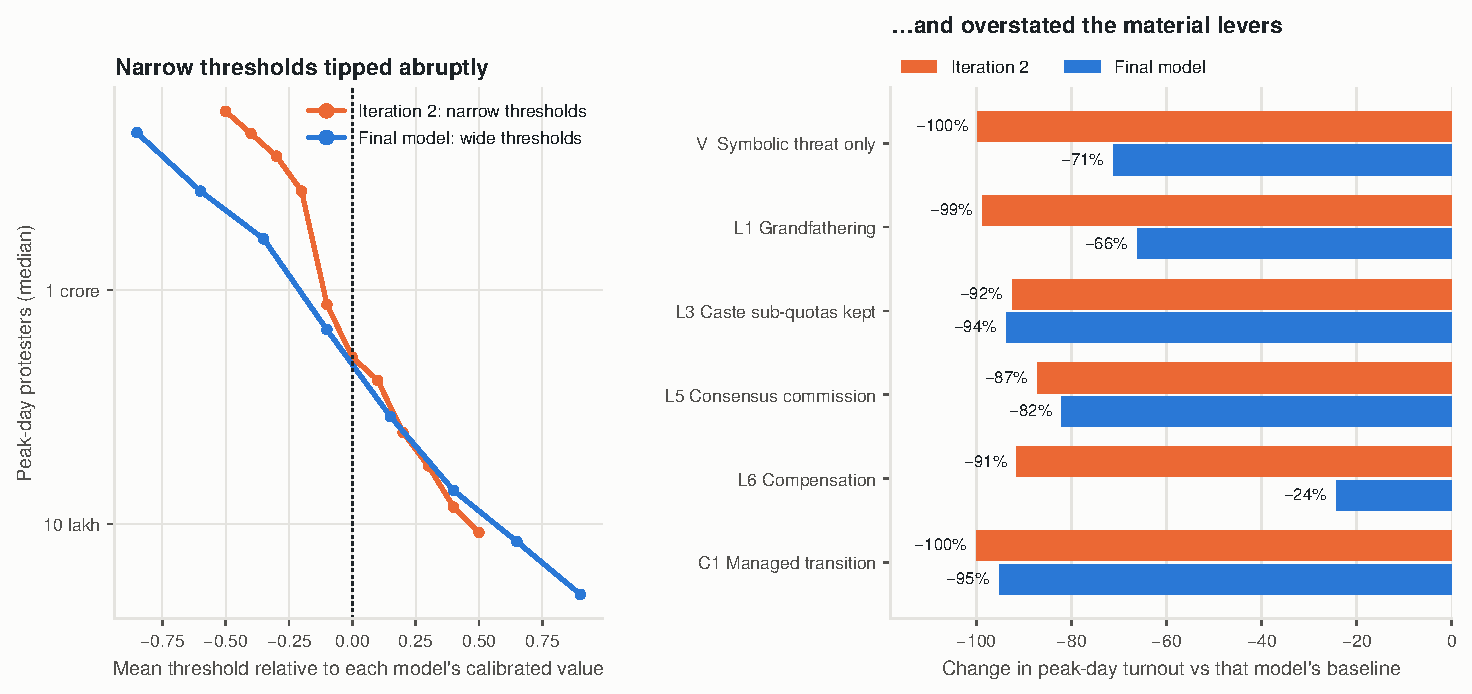
\includegraphics[width=\linewidth]{../figures/fig08_model_development.pdf}
\caption{Left: peak turnout against mean threshold, centred on each model's calibrated value. Iteration 2 drops about threefold in a single 0.1 step just below its calibrated value; the final model declines steadily. Right: iteration 2 overstated material levers (grandfathering, compensation) and understated symbolic-only protest.}
\label{fig:development}
\end{figure}

\subsection{Lessons}
\begin{enumerate}
\item \textbf{Calibration is not validation.} Iteration 2 matched the turnout target but could not reproduce a well-documented episode. A validation test built from a qualitatively different case, here a shock with no material loss, exposed it.
\item \textbf{Bound every positive feedback.} Unbounded contagion guarantees runaway behaviour.
\item \textbf{Threshold heterogeneity is a substantive assumption.} It determines whether interventions look marginal or miraculous.
\item \textbf{Some parameters are not separately identified.} For losses, only the product $\lambda w_m$ enters grievance, so the model cannot distinguish stronger loss aversion from a heavier material weight (Section~\ref{sec:robustness}).
\end{enumerate}

\section{Calibration and validation}
\label{sec:calibration}

\paragraph{Calibration target} The target for the baseline peak is 20 lakh to 1 crore. It comes from an independent back-of-envelope estimate, not from the model:
\begin{itemize}
\item bandh-day participation of 0.5--2\% among India's roughly 37 crore SC and ST people;
\item 0.1--0.5\% among OBC people, whose separate quota would disappear.
\end{itemize}
The benchmarks for this estimate are the 2018 bandh and the Maratha marches, whose largest single event drew 3--5 lakh in one city. The mean threshold $\bar\theta$ is the only parameter tuned to the target. At $\bar\theta=\ParamMeanThreshold$ the baseline peak is \PeakCentralBaseline{} (Figure~\ref{fig:response}).

\paragraph{Validation} Four checks were made against stylized facts, none of which were used in calibration.
\begin{enumerate}
\item A symbolic-only shock produces \PeakCentralSymbolicOnlyValidation{} on the peak day (S1).
\item Turnout spikes on bandh-call days and decays between them (S2).
\item SC agents dominate turnout while General agents do not protest (Figure~\ref{fig:groups}).
\item Deaths are of the same order as 2018: a median of \DeathsCentralBaseline{} over 40 days, against 11--14 on the single day in 2018 (S5).
\end{enumerate}

\begin{figure}[H]
\centering
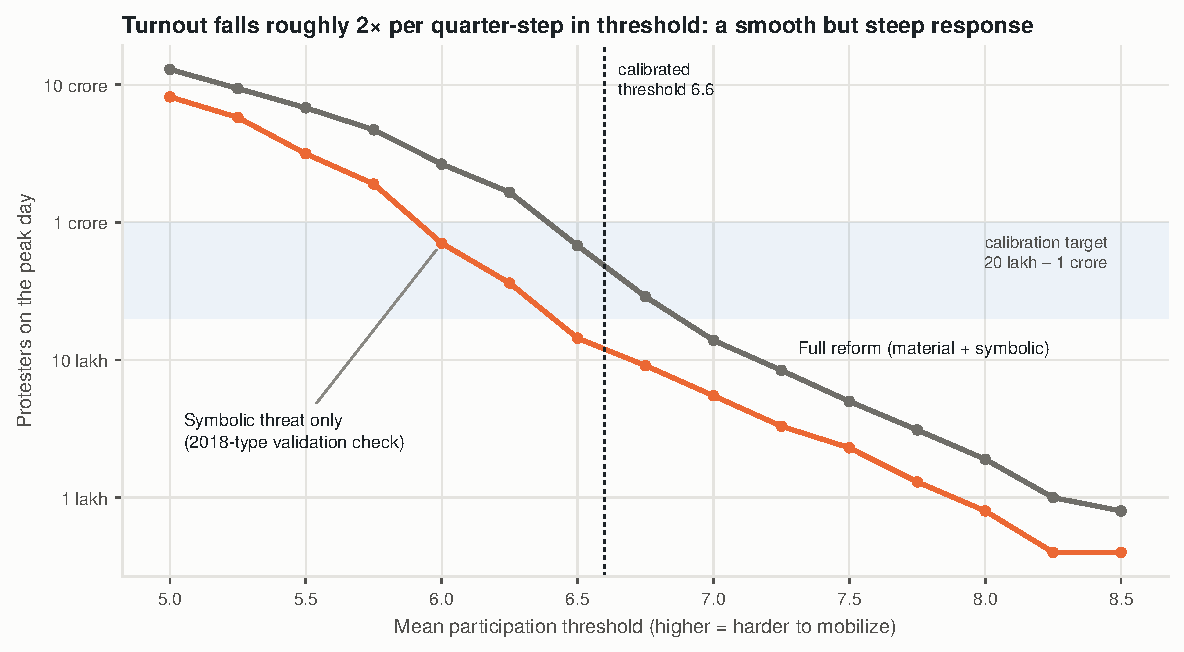
\includegraphics[width=0.9\linewidth]{../figures/fig05_threshold_response_curve.pdf}
\caption{Final model: peak-day turnout against mean threshold, for the full reform and for the symbolic-only validation shock (6 runs per point).}
\label{fig:response}
\end{figure}

\section{Experimental design}
\label{sec:design}

Table~\ref{tab:scenarios} maps each scenario to its parameter changes. Every scenario was run 50 times with paired draws in two regimes: the central regime, and a high-mobilization regime with $\bar\theta$ lowered by 0.5, which raises baseline turnout about 4.5-fold. The outcomes are:
\begin{itemize}
\item peak-day protesters (the busiest single day);
\item cumulative unique participants over the 40-day campaign;
\item total deaths.
\end{itemize}
We report medians and 10th--90th percentile intervals.

\begin{table}[H]
\centering\small
\caption{Scenarios and how they enter the model.}
\label{tab:scenarios}
\begin{tabularx}{\linewidth}{@{}lLL@{}}
\toprule
Code & Scenario & Parameter changes\\
\midrule
Base & Abrupt \rupee8L income-only switch & None\\
V & Symbolic threat only (validation) & All $m_i=0$\\
L1 & Grandfather current cohorts, 10-year glide & All material losses ×0.3; $s_g$×0.95\\
L2 & Expand seats so no group loses & Below-line SC/ST/OBC losses set to 0\\
L3 & Keep caste sub-quotas, income filter inside & $s_g$×0.4 for SC/ST/OBC; below-line losses 0\\
L4 & Sub-classify to favour most-deprived & Most-deprived tier: $m_i-0.5$; symbolic share 0.3\\
L5 & Data-first commission, cross-party consensus & $a$: 1.5→1.0; $s_g$×0.8\\
L6 & Compensate above-line losers & Above-line SC/ST loss ×0.5\\
L7 & Guarantee untouched protections & $s_g$×0.85\\
B1 & Internet shutdowns & $\beta_n,\beta_v$×0.6; bandh $b_t$×0.8; $\kappa$×2.5\\
B2 & Heavy policing and mass arrests & $c_t=0.4$ on bandh days; $\kappa$×3; $\delta$×1.5\\
C1 & Managed transition & L1+L2+L5+L6+L7\\
C2 & Hybrid package & L3+L4+L1+L5+L6+L7\\
\bottomrule
\end{tabularx}
\end{table}

\section{Results}
\label{sec:results}

\subsection{The abrupt switch}
An abrupt switch produces a median peak of \PeakCentralBaseline{}, with an 80\% interval of \PeakRangeCentralBaseline{} lakh. Over 40 days, \CumulativeCentralBaseline{} people protest at least once, and there are a median of \DeathsCentralBaseline{} deaths. In the high-mobilization regime the peak is \PeakHighBaseline{}.

Figure~\ref{fig:grievance} decomposes grievance. Symbolic threat is the larger component for every segment except SC and ST families above the line, who are under 3\% of the population. SC agents dominate turnout (Figure~\ref{fig:groups}) because they combine the highest symbolic threat, the strongest organization and the largest group of direct losers.

\begin{figure}[H]
\centering
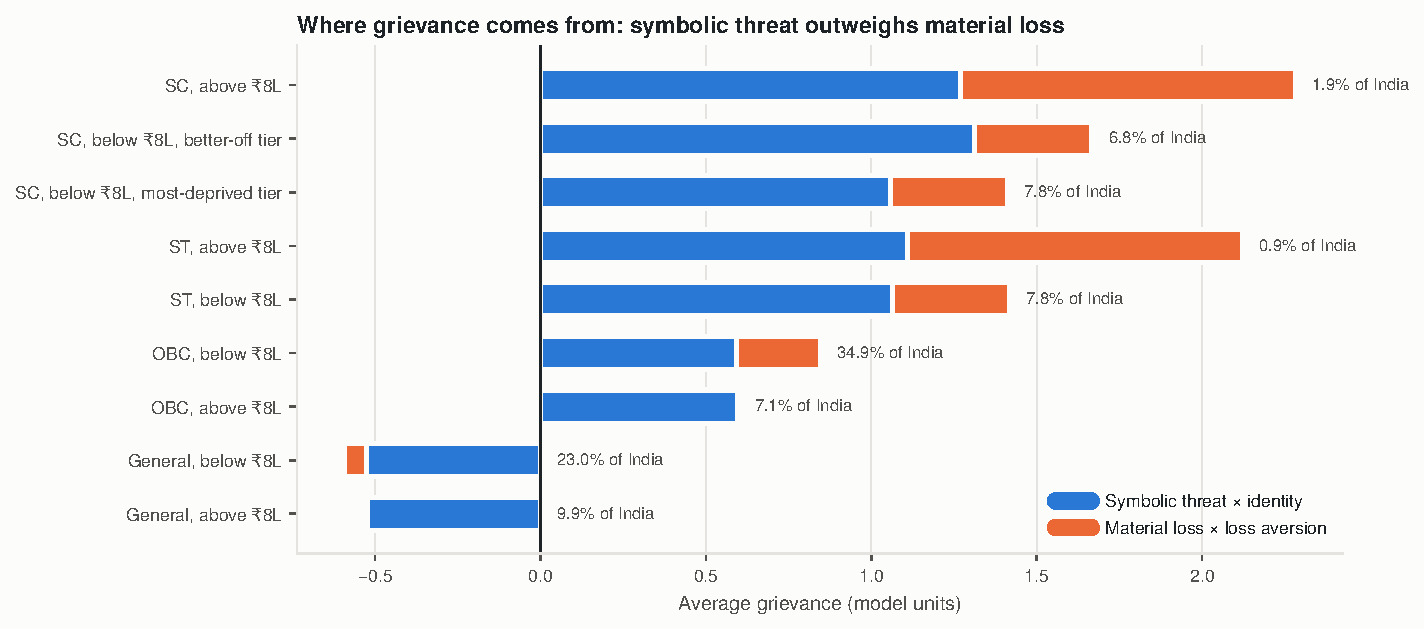
\includegraphics[width=0.88\linewidth]{../figures/fig04_grievance_composition.pdf}
\caption{Mean grievance by segment, split into symbolic and material components (baseline).}
\label{fig:grievance}
\end{figure}

\begin{figure}[H]
\centering
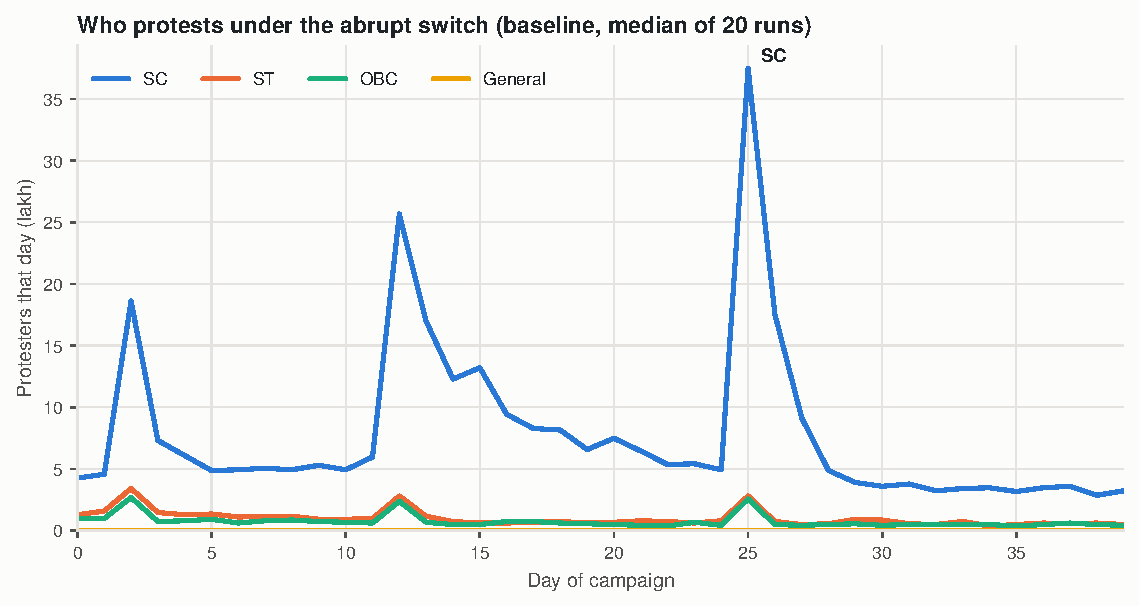
\includegraphics[width=0.85\linewidth]{../figures/fig03_turnout_by_group.pdf}
\caption{Baseline daily turnout by group (median of 20 runs).}
\label{fig:groups}
\end{figure}

\subsection{Interventions}
Figure~\ref{fig:ranking} and Table~\ref{tab:central} report all scenarios. Table~\ref{tab:hypotheses} summarizes the verdict on each hypothesis.

\begin{figure}[H]
\centering
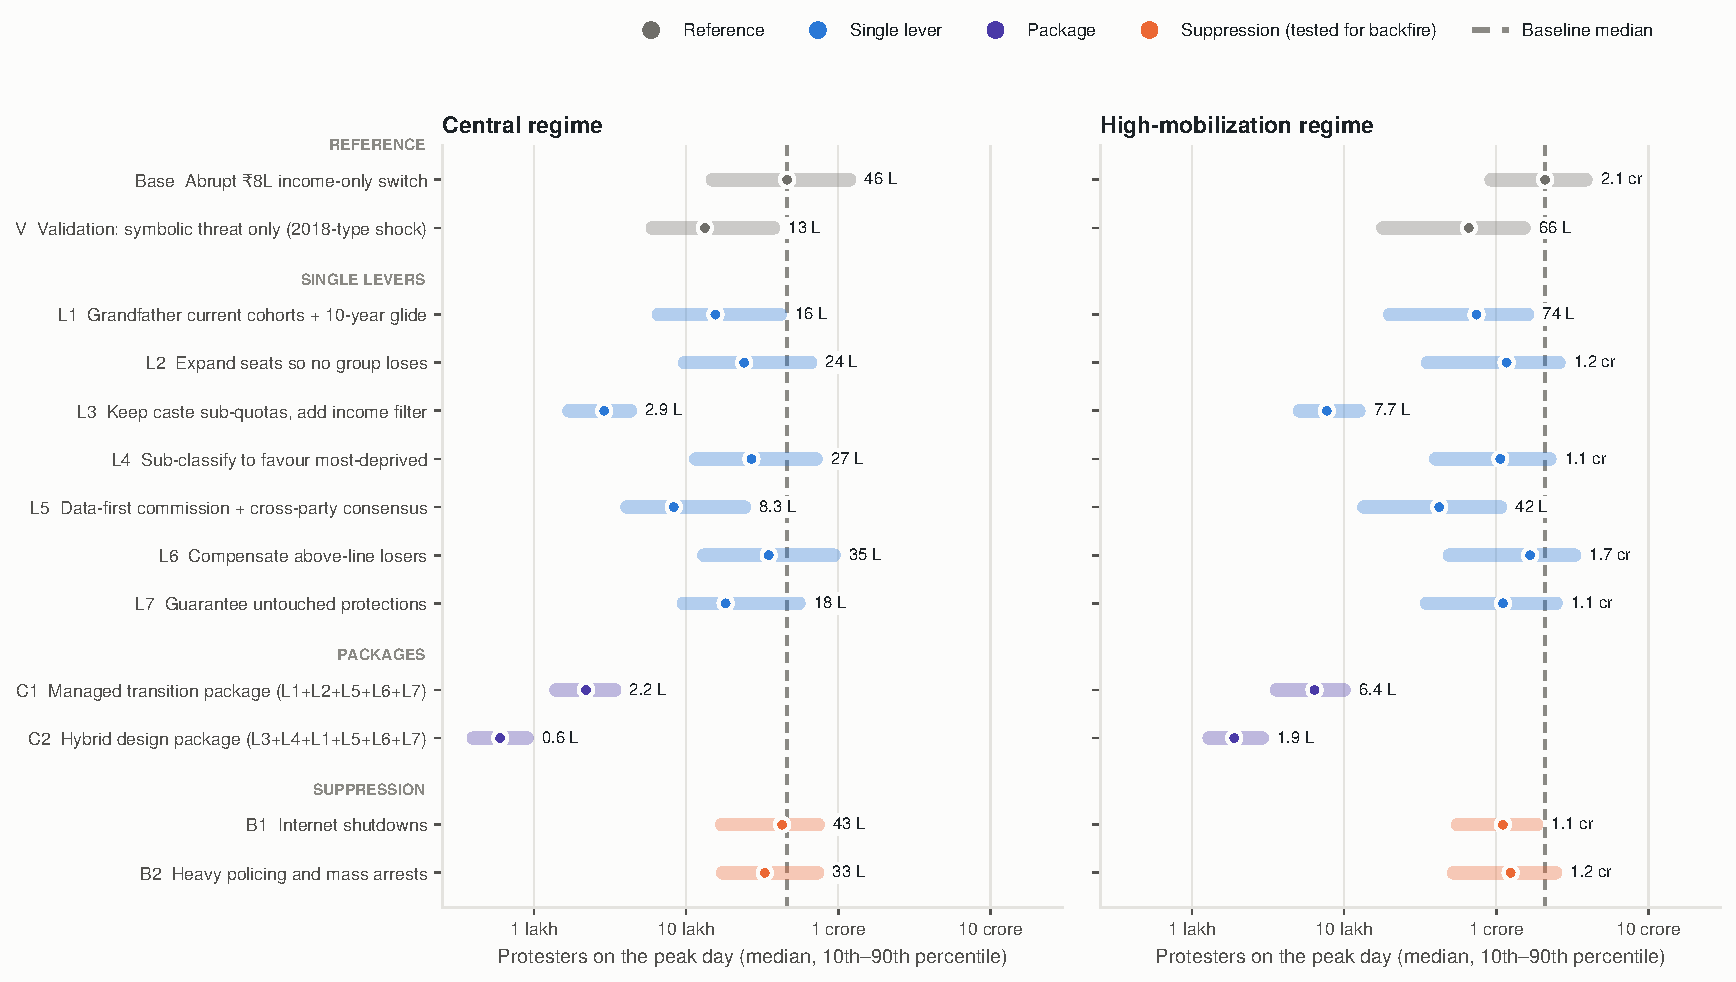
\includegraphics[width=\linewidth]{../figures/fig01_intervention_ranking.pdf}
\caption{Peak-day protesters by scenario and regime (median of 50 paired runs; bars show 10th--90th percentile).}
\label{fig:ranking}
\end{figure}

\begin{table}[H]
\centering\small
\caption{Central regime. Peak in lakh; cumulative in crore; 50 paired runs.}
\label{tab:central}
\begin{tabularx}{\linewidth}{@{}lLrrrrr@{}}
\toprule
 & Scenario & Peak & 10th--90th & Change & Ever protest & Deaths\\
\midrule
\tablerows{../report/generated/scenario_table_central.tex}
\bottomrule
\end{tabularx}
\end{table}

\paragraph{Symbolic levers dominate} Keeping caste sub-quotas with an income filter inside them (L3) is the strongest single lever: \PeakChangeCentralHybridCasteSubquotas{} in the central regime and \PeakChangeHighHybridCasteSubquotas{} in the high-mobilization regime. Credible guarantees (L7) reduce symbolic threat by only 15\% but cut turnout by \PeakChangeCentralCredibleGuarantees{}. The threshold response amplifies any reduction in symbolic grievance, which is the largest component for most of the mobilizable population.

\paragraph{Process is the strongest end-state-preserving lever} The consensus commission (L5) reduces the opposition-party amplifier by a third and symbolic threat by a fifth, cutting turnout by \PeakChangeCentralConsensusCommission{}. It works mainly on bandh days, which set the peak.

\paragraph{Material levers are weaker} Grandfathering (L1) reduces turnout by \PeakChangeCentralGrandfathering{}, close to the symbolic-only floor of \PeakCentralSymbolicOnlyValidation{}. It removes most material grievance but none of the symbolic grievance. Seat expansion (L2) helps less (\PeakChangeCentralSeatExpansion{}) because the below-line loss is thin per person. Compensation (L6) is weakest (\PeakChangeCentralCompensation{}), because it targets under 3\% of the population and does not touch symbolic threat. This inverts the prominence of compensation in the retrenchment literature, a point we return to in Section~\ref{sec:discussion}.

\paragraph{Coalition splitting is partial} Sub-classification (L4) removes the most-deprived tier from the protest but leaves the better-off tier, which contains nearly all direct losers, mobilized. The result is \PeakChangeCentralSubClassification{}.

\paragraph{Packages compound} The managed transition (C1) keeps the income-only end state and reaches \PeakCentralManagedTransition{} (\PeakChangeCentralManagedTransition{}). The hybrid package (C2) reaches \PeakCentralHybridPackage{} (\PeakChangeCentralHybridPackage{}). Because turnout is convex in net motivation, the combined effects exceed what the individual effects would suggest.

\subsection{Suppression}
\begin{itemize}
\item \textbf{Internet shutdowns (B1)} reduce the central-regime peak by only \PeakChangeCentralInternetShutdown{}, raise cumulative participation by \CumulativeChangeCentralInternetShutdown{}, and multiply deaths by \DeathRatioCentralInternetShutdown{}.
\item \textbf{Heavy policing (B2)} reduces the peak by \PeakChangeCentralHeavyPolicing{} but raises cumulative participation by \CumulativeChangeCentralHeavyPolicing{} and multiplies deaths by \DeathRatioCentralHeavyPolicing{}.
\end{itemize}
Figure~\ref{fig:paths} shows the mechanism. Policing flattens the bandh-day spikes, but the martyr effect sustains higher turnout between bandhs. In the high-mobilization regime both measures cut the peak more (B1 \PeakChangeHighInternetShutdown{}, B2 \PeakChangeHighHeavyPolicing{}), but deaths still rise by factors of \DeathRatioHighInternetShutdown{} and \DeathRatioHighHeavyPolicing{}. H8 and H9 are rejected as mitigation strategies: at best they trade turnout for lives.

\begin{figure}[H]
\centering
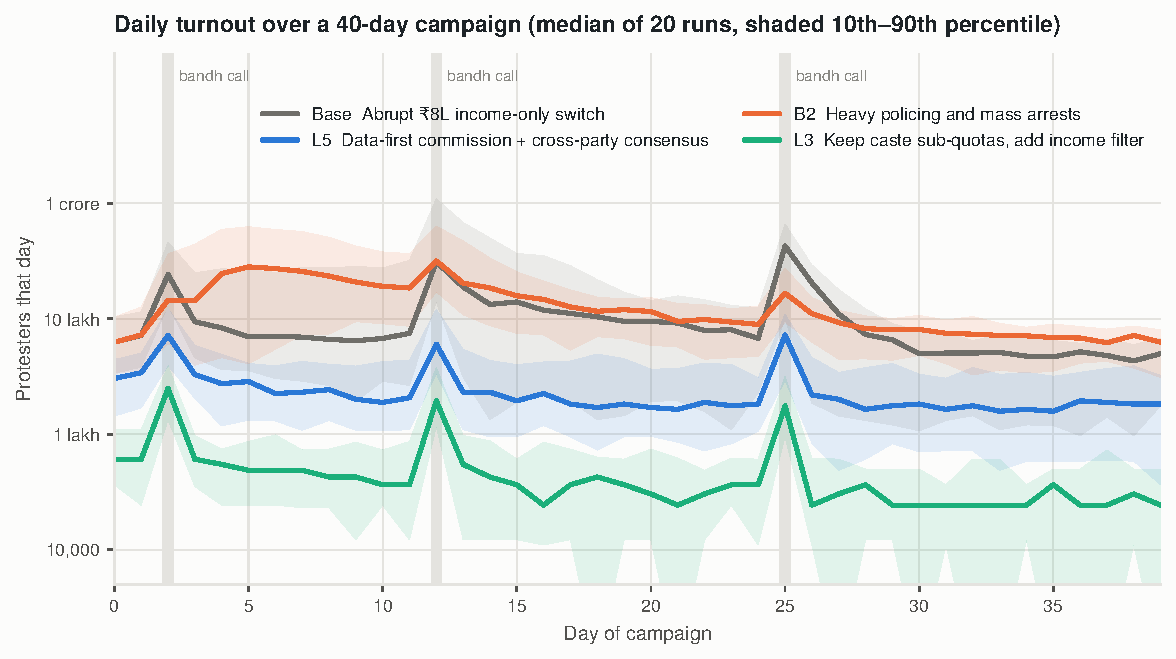
\includegraphics[width=0.9\linewidth]{../figures/fig02_daily_turnout_paths.pdf}
\caption{Daily turnout for four scenarios (median of 20 runs; shaded 10th--90th percentile).}
\label{fig:paths}
\end{figure}

\begin{figure}[H]
\centering
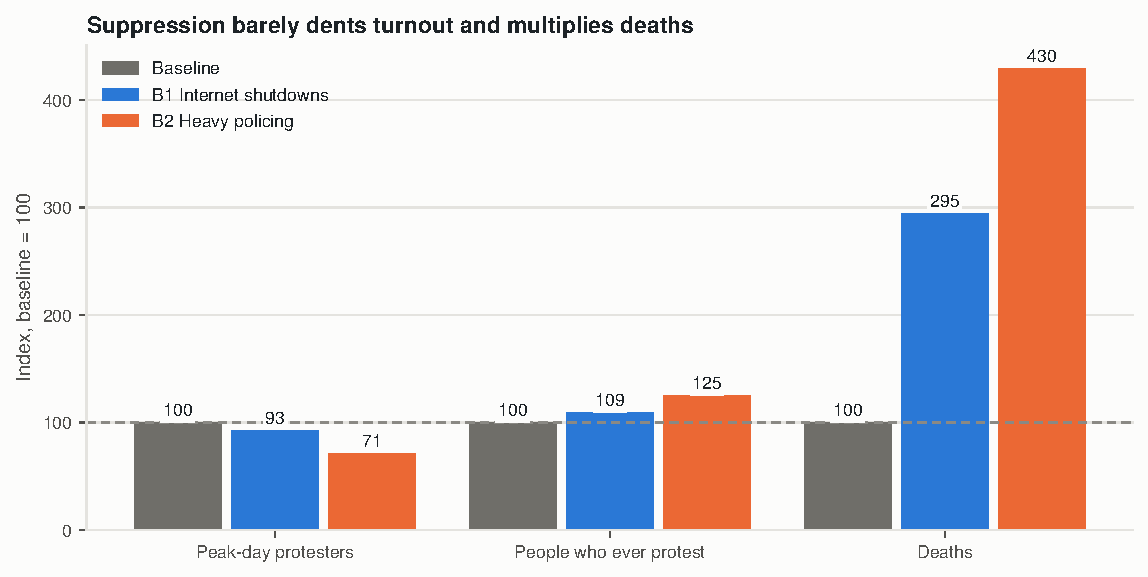
\includegraphics[width=0.8\linewidth]{../figures/fig06_suppression_backfire.pdf}
\caption{Suppression outcomes indexed to the baseline (= 100), central regime.}
\label{fig:suppression}
\end{figure}

\begin{table}[H]
\centering\small
\caption{Hypothesis verdicts (central regime, change in peak-day turnout).}
\label{tab:hypotheses}
\begin{tabularx}{\linewidth}{@{}lLrl@{}}
\toprule
 & Hypothesis & Change & Verdict\\
\midrule
H1 & Grandfathering and glide path & \PeakChangeCentralGrandfathering & Supported\\
H2 & Seat expansion & \PeakChangeCentralSeatExpansion & Partly supported\\
H3 & Caste sub-quotas with income filter & \PeakChangeCentralHybridCasteSubquotas & Strongly supported\\
H4 & Sub-classification & \PeakChangeCentralSubClassification & Partly supported\\
H5 & Consensus commission & \PeakChangeCentralConsensusCommission & Strongly supported\\
H6 & Compensation & \PeakChangeCentralCompensation & Weak\\
H7 & Credible guarantees & \PeakChangeCentralCredibleGuarantees & Supported\\
H8 & Internet shutdowns reduce protest & \PeakChangeCentralInternetShutdown & Rejected (deaths ×\DeathRatioCentralInternetShutdown)\\
H9 & Heavy policing reduces protest & \PeakChangeCentralHeavyPolicing & Rejected (deaths ×\DeathRatioCentralHeavyPolicing)\\
\bottomrule
\end{tabularx}
\end{table}

\section{Robustness and sensitivity}
\label{sec:robustness}

\paragraph{Hybrid sensitivity} The hybrid's effect rests on the assumption that retaining caste categories removes 60\% of symbolic threat. The 2024 bandh, triggered by a mere suggestion of an SC/ST creamy layer, is reason for caution. Leaving 40\%, 60\% and 80\% of symbolic threat in place yields peaks of \HybridRetainedForty{}, \HybridRetainedSixty{} and \HybridRetainedEighty{}. Even the weakest version cuts turnout by about 80\%, because the hybrid also removes the pool-merger loss for the below-line majority.

\paragraph{Leave-one-out} Removing each component of the managed transition in turn gives the following peaks:
\begin{itemize}
\item full package: \ManagedTransitionFull{};
\item without the consensus commission: \ManagedTransitionWithoutBuildConsensusThroughDataFirstCommission{};
\item without guarantees: \ManagedTransitionWithoutGuaranteeUntouchedProtections{};
\item without grandfathering: \ManagedTransitionWithoutGrandfatherCurrentCohortsWithTenYearGlide{};
\item without seat expansion: \ManagedTransitionWithoutExpandSeatsSoNoGroupLoses{};
\item without compensation: \ManagedTransitionWithoutCompensateAboveLineLosers{}.
\end{itemize}
Consensus carries the package; compensation contributes almost nothing.

\begin{figure}[H]
\centering
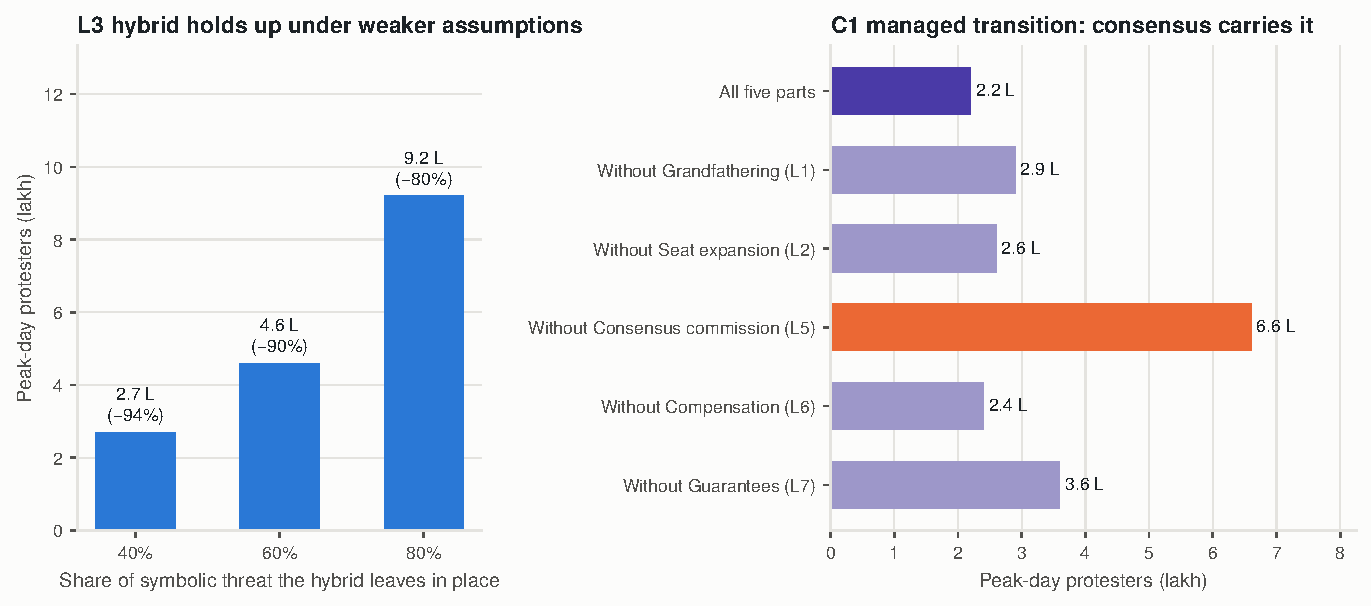
\includegraphics[width=\linewidth]{../figures/fig07_robustness_checks.pdf}
\caption{Hybrid sensitivity (left) and managed-transition leave-one-out (right), 30 paired runs each.}
\end{figure}

\paragraph{One-at-a-time sensitivity} Each of twelve parameters was perturbed by $\pm25\%$, or by $\pm0.25$ for $\bar\theta$. For each of the \SensPerturbationCount{} perturbed worlds, the baseline was re-run with 20 runs and the nine levers and packages with 10 runs each. The reference baseline under this design is \SensReferencePeak{}.

Baseline turnout is most sensitive to the \SensWidestParameter{}, ranging from \SensWidestLow{} to \SensWidestHigh{} (Figure~\ref{fig:tornado}). The ranking of interventions is far more stable than their magnitudes:
\begin{itemize}
\item the Spearman correlation between the perturbed and reference rankings has a median of \SensRankCorrMedian{} and a minimum of \SensRankCorrMin{};
\item L3 is the strongest single lever in \SensHybridStrongestCount{} of \SensPerturbationCount{} perturbations;
\item the weakest single lever is \SensWeakestSummary{} of the \SensPerturbationCount{} perturbations.
\end{itemize}
As noted in Section~\ref{sec:development}, lowering $\lambda$ and lowering $w_m$ give identical results, because they enter only as a product.

\begin{figure}[H]
\centering
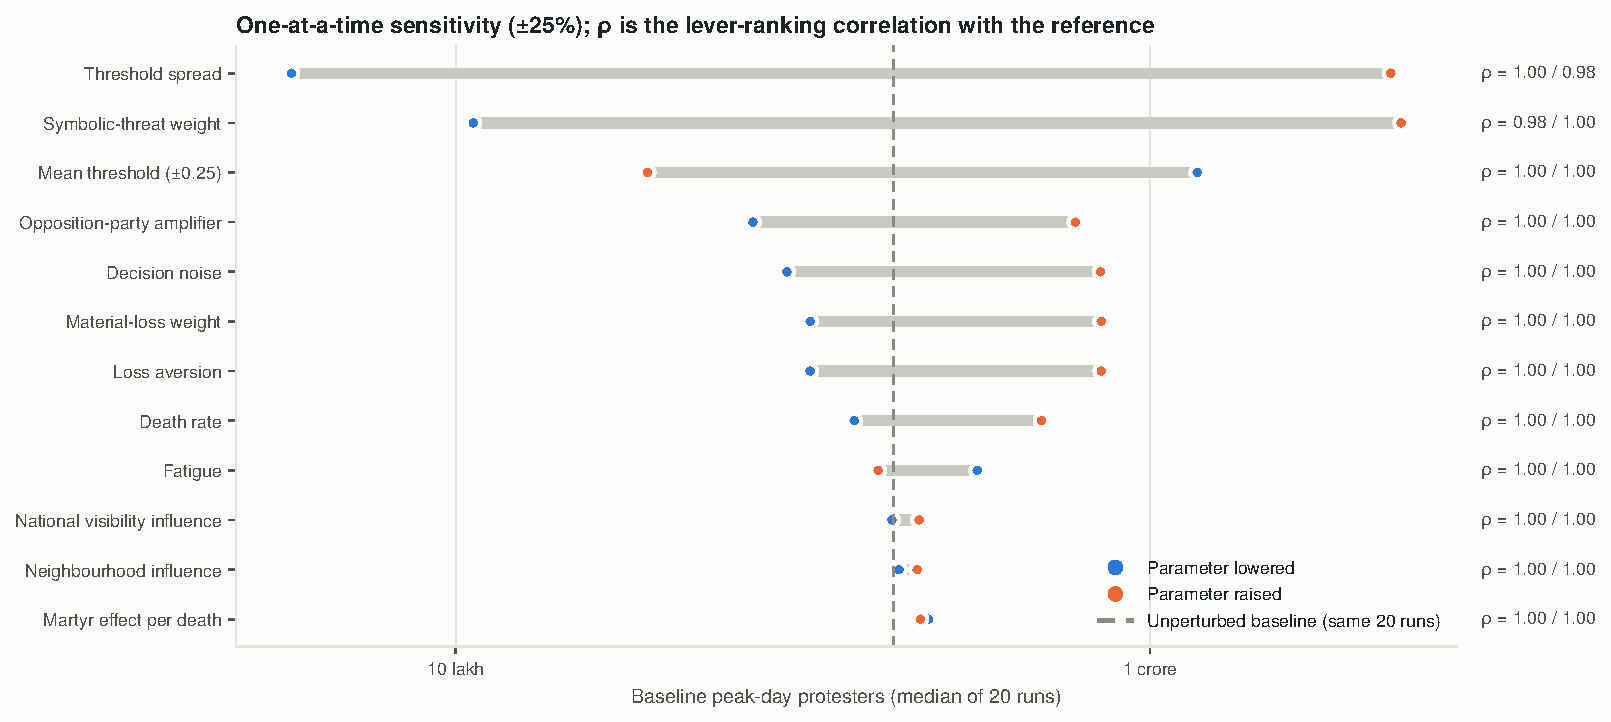
\includegraphics[width=0.95\linewidth]{../figures/fig09_sensitivity_tornado.pdf}
\caption{Baseline peak under $\pm25\%$ perturbations. $\rho$ is the Spearman correlation of the nine-lever ranking with the reference, shown as lowered / raised.}
\label{fig:tornado}
\end{figure}

\begin{table}[H]
\centering\small
\caption{Sensitivity detail. Peaks in lakh (20 runs); $\rho$ for lowered and raised parameter; strongest and weakest single lever (lowered/raised).}
\begin{tabular}{@{}lrrrrll@{}}
\toprule
Parameter & Lowered & Raised & $\rho_-$ & $\rho_+$ & Strongest & Weakest\\
\midrule
\tablerows{generated/sensitivity_rows.tex}
\bottomrule
\end{tabular}
\end{table}

\paragraph{Agent-count convergence} Table~\ref{tab:convergence} re-runs the baseline and the hybrid at four population sizes, from 30{,}000 to 240{,}000 agents. Medians show no systematic trend with agent count, and their differences are small next to the order-of-magnitude spread between runs. The hybrid's effect is stable at every size. The discretization does not drive the findings.

\begin{table}[H]
\centering\small
\caption{Agent-count convergence (20 paired runs each).}
\label{tab:convergence}
\begin{tabular}{@{}rrrrr@{}}
\toprule
Agents & People per agent & Baseline peak (lakh) & 10th--90th & Hybrid peak (lakh)\\
\midrule
\tablerows{generated/convergence_rows.tex}
\bottomrule
\end{tabular}
\end{table}

\section{Discussion}
\label{sec:discussion}

\paragraph{Why symbolic levers dominate} In the model, as in 2018, most of the mobilizable grievance is symbolic. Material loss is concentrated on a small group; symbolic threat is spread across the 37 crore people of SC and ST communities and part of the OBC population. Levers that address recognition therefore act on the bulk of potential participants, and the convex threshold response multiplies their effect. This is why a 15\% cut in symbolic threat (L7) outperforms halving the material loss of the direct losers (L6) by a wide margin.

\paragraph{Compensation and the retrenchment literature} \citet{pierson1994} emphasizes compensation as a blame-avoidance tool. Our results suggest its value depends on how grievance is composed. Where losses are material and the losers are the mobilizers, as with pensioners in welfare retrenchment, compensation addresses the grievance. Where the mobilizing grievance is symbolic and the material losers are a small minority, it does not. Blame-sharing through consensus, the other Pierson strategy, transfers well.

\paragraph{Policy implications} Four implications follow, conditional on the model.
\begin{enumerate}
\item Whether caste stays a criterion matters more than any compensation scheme. An income filter inside caste categories achieves income targeting at a small fraction of the unrest.
\item If the income-only end state is the goal, sequencing and ownership matter most: data first, then a commission with opposition representation, then a phased and grandfathered transition with statutory guarantees.
\item Suppression is not a mitigation strategy. Consistent with India's own record on shutdowns \citep{rydzak2019}, it trades a lower peak for more deaths and, in the case of policing, more total participation.
\item Because levers compound, partial measures should be evaluated as a package, not one at a time.
\end{enumerate}

\paragraph{Feasibility} The most effective end-state-preserving lever, cross-party consensus, is also the hardest to obtain. Reservation is electorally central, and opposition parties may gain from mobilizing against a reform. The model treats consensus as exogenous; endogenizing party strategy is a natural extension.

\section{Limitations and threats to validity}
\label{sec:limitations}
\begin{itemize}
\item \textbf{Construct validity.} Grievance weights, intervention effects and organizational capacities are assumptions informed by qualitative evidence, not estimates from Indian protest data. The intervention mappings in Table~\ref{tab:scenarios} are the model's most consequential untested assumptions.
\item \textbf{Calibration target.} The 20 lakh--1 crore target is itself an estimate. Reported turnout for Indian bandhs is unreliable.
\item \textbf{Identification.} Material weight and loss aversion are not separately identified, and symbolic weight and group threat levels trade off against the mean threshold.
\item \textbf{Omitted structure.} Neighbourhoods are single-group, and there is no geography, regional variation, counter-mobilization, media dynamics, courts or electoral feedback. OBC heterogeneity is not represented.
\item \textbf{Horizon.} Campaigns run 40 days with fixed bandh calls. Long-run political consequences, including electoral punishment, are outside the model.
\item \textbf{Magnitudes versus ranking.} The sensitivity analysis supports the ranking of interventions much more strongly than any specific turnout figure.
\end{itemize}

\section{Ethics statement}
\label{sec:ethics}
The study uses no individual-level data; the population is synthetic and built from published aggregate shares. Suppression tactics are included only to test whether they backfire, and they are not presented as options. Obfuscation, which is manipulating what citizens know about a reform, is deliberately excluded from the intervention set. The model is not a forecast of any actual policy. It is intended to inform the design of reforms that respect democratic contestation, not to help any actor suppress it.

\section{Reproducibility}
\label{sec:reproducibility}
All code, results, figures and videos are available at \href{https://github.com/utsavbalhara/reservation-reform-protest-model}{github.com/utsavbalhara/\allowbreak reservation-reform-protest-model}. Seeds are fixed. Every number in this paper is generated from the result files into LaTeX macros; none is typed by hand. The main commands are:
\begin{small}
\begin{verbatim}
python -m experiments.compare_interventions --regime central
python -m experiments.compare_interventions --regime high-mobilization
python -m experiments.check_robustness
python -m experiments.calibrate_participation_threshold
python -m experiments.record_daily_trajectories
python -m experiments.replay_model_development
python -m experiments.sensitivity_analysis
python -m visualization.render_result_figures
python -m visualization.render_paper_figures
python -m visualization.write_latex_result_macros
python -m visualization.write_paper_macros
\end{verbatim}
\end{small}

\section*{Acknowledgements}
Model development, coding and drafting were carried out with the assistance of Claude (Anthropic), an AI system. All design decisions, interpretations and remaining errors are the author's.

\begin{thebibliography}{99}
\bibitem[Bharti(2018)]{bharti2018} Bharti, N.~K. (2018). Wealth inequality, class and caste in India, 1961--2012. WID.world Working Paper 2018/14.
\bibitem[Davenport(2007)]{davenport2007} Davenport, C. (2007). State repression and political order. \emph{Annual Review of Political Science}, 10, 1--23.
\bibitem[Deshpande(2013)]{deshpande2013} Deshpande, A. (2013). \emph{Affirmative Action in India}. Oxford University Press.
\bibitem[Epstein(2002)]{epstein2002} Epstein, J.~M. (2002). Modeling civil violence: An agent-based computational approach. \emph{Proceedings of the National Academy of Sciences}, 99(suppl.~3), 7243--7250.
\bibitem[Galanter(1984)]{galanter1984} Galanter, M. (1984). \emph{Competing Equalities: Law and the Backward Classes in India}. University of California Press.
\bibitem[Granovetter(1978)]{granovetter1978} Granovetter, M. (1978). Threshold models of collective behavior. \emph{American Journal of Sociology}, 83(6), 1420--1443.
\bibitem[Hess and Martin(2006)]{hess2006} Hess, D., \& Martin, B. (2006). Repression, backfire, and the theory of transformative events. \emph{Mobilization}, 11(2), 249--267.
\bibitem[Kahneman and Tversky(1979)]{kahneman1979} Kahneman, D., \& Tversky, A. (1979). Prospect theory: An analysis of decision under risk. \emph{Econometrica}, 47(2), 263--291.
\bibitem[Lichbach(1987)]{lichbach1987} Lichbach, M.~I. (1987). Deterrence or escalation? The puzzle of aggregate studies of repression and dissent. \emph{Journal of Conflict Resolution}, 31(2), 266--297.
\bibitem[McAdam(1982)]{mcadam1982} McAdam, D. (1982). \emph{Political Process and the Development of Black Insurgency, 1930--1970}. University of Chicago Press.
\bibitem[McCarthy and Zald(1977)]{mccarthy1977} McCarthy, J.~D., \& Zald, M.~N. (1977). Resource mobilization and social movements: A partial theory. \emph{American Journal of Sociology}, 82(6), 1212--1241.
\bibitem[PIB(2025)]{pib2025} Press Information Bureau, Government of India (2025). Census 2027: India's first digital enumeration exercise. Cabinet approval of the scheme for conduct of Census of India 2027, including caste enumeration.
\bibitem[Pierson(1994)]{pierson1994} Pierson, P. (1994). \emph{Dismantling the Welfare State? Reagan, Thatcher, and the Politics of Retrenchment}. Cambridge University Press.
\bibitem[Pierson(1996)]{pierson1996} Pierson, P. (1996). The new politics of the welfare state. \emph{World Politics}, 48(2), 143--179.
\bibitem[PRICE(2023)]{price2023} People Research on India's Consumer Economy (2023). ICE 360° survey: income distribution by social group.
\bibitem[Rydzak(2019)]{rydzak2019} Rydzak, J. (2019). Of blackouts and bandhs: The strategy and structure of disconnected protest in India. SSRN Working Paper 3330413.
\bibitem[Rydzak et~al.(2020)]{rydzak2020} Rydzak, J., Karanja, M., \& Opiyo, N. (2020). Dissent does not die in darkness: Network shutdowns and collective action in African countries. \emph{International Journal of Communication}, 14, 4264--4287.
\bibitem[Schelling(1978)]{schelling1978} Schelling, T.~C. (1978). \emph{Micromotives and Macrobehavior}. W.~W.~Norton.
\bibitem[Tajfel and Turner(1979)]{tajfel1979} Tajfel, H., \& Turner, J.~C. (1979). An integrative theory of intergroup conflict. In W.~G. Austin \& S.~Worchel (Eds.), \emph{The Social Psychology of Intergroup Relations} (pp.~33--47). Brooks/Cole.
\bibitem[Tarrow(1994)]{tarrow1994} Tarrow, S. (1994). \emph{Power in Movement: Social Movements, Collective Action and Politics}. Cambridge University Press.
\bibitem[The Tribune(2022)]{tribune2022} The Tribune (2022). 2.14 lakh additional seats to be created in central educational institutions, Centre tells SC.
\bibitem[Tversky and Kahneman(1992)]{tversky1992} Tversky, A., \& Kahneman, D. (1992). Advances in prospect theory: Cumulative representation of uncertainty. \emph{Journal of Risk and Uncertainty}, 5(4), 297--323.
\bibitem[Watts(2002)]{watts2002} Watts, D.~J. (2002). A simple model of global cascades on random networks. \emph{Proceedings of the National Academy of Sciences}, 99(9), 5766--5771.
\bibitem[Weaver(1986)]{weaver1986} Weaver, R.~K. (1986). The politics of blame avoidance. \emph{Journal of Public Policy}, 6(4), 371--398.
\end{thebibliography}

\subsection*{Cases and statutes}
{\small
\emph{Indra Sawhney v.\ Union of India}, 1992 Supp (3) SCC 217. \emph{Ashoka Kumar Thakur v.\ Union of India}, (2008) 6 SCC 1. \emph{Subhash Kashinath Mahajan v.\ State of Maharashtra}, (2018) 6 SCC 454. \emph{Janhit Abhiyan v.\ Union of India}, Supreme Court of India, 7 November 2022. \emph{State of Punjab v.\ Davinder Singh}, Supreme Court of India, 1 August 2024. The Constitution (One Hundred and Third Amendment) Act, 2019. The Scheduled Castes and the Scheduled Tribes (Prevention of Atrocities) Amendment Act, 2018. Brazil, Law No.\ 12.711 of 29 August 2012.\par}

\appendix
\section{High-mobilization regime}
\begin{table}[H]
\centering\small
\caption{High-mobilization regime ($\bar\theta$ lowered by 0.5), 50 paired runs.}
\begin{tabularx}{\linewidth}{@{}lLrrrrr@{}}
\toprule
 & Scenario & Peak & 10th--90th & Change & Ever protest & Deaths\\
\midrule
\tablerows{../report/generated/scenario_table_high-mobilization.tex}
\bottomrule
\end{tabularx}
\end{table}

\section{Code map}
\begin{tabularx}{\linewidth}{@{}lL@{}}
\toprule
File & Contents\\
\midrule
\texttt{synthetic\_population.py} & Population construction, tiers, income line, neighbourhoods\\
\texttt{model\_parameters.py} & Parameter dataclass and calibrated baseline\\
\texttt{protest\_campaign.py} & Daily dynamics: grievance, contagion, decision, fatigue, deaths\\
\texttt{parameter\_uncertainty.py} & Monte Carlo world draws\\
\texttt{policy\_interventions.py} & Interventions and scenario catalogue\\
\texttt{monte\_carlo.py} & Paired runs and summaries\\
\texttt{replay\_model\_development.py} & Iterations 1--3 re-run with current code\\
\texttt{sensitivity\_analysis.py} & One-at-a-time sensitivity, rank stability, convergence\\
\bottomrule
\end{tabularx}

\end{document}
